\section{NLP}

\ac{NLP} bezeichnet Technologien, mit deren Hilfe Texte oder Sprache in strukturierte Informationen codiert werden kann. Sie vereint die Forschungsgebiete künstliche Intelligenz in der Computerwissenschaft und Linguistik (\cite[vgl.][1]{ITWISSEN}). Ziel ist es, Tools zu entwickeln, die menschliche Sprache erlernen, verstehen und sogar generieren können. Stetig wachsende Hardwareressourcen, die große Zahl zur Verfügung stehender linguistischer Daten und der wissenschaftliche Fortschritte in Computerwissenschaft und Lignuistik tragen dazu bei, dass die Anzahl der \ac{NLP} Anwendungsfälle in den letzten Jahren stark angestiegen ist (\cite[vgl.][1]{HIRSCHBERG}). 
\par
Zu den wichtigsten Aufgaben des \ac{NLP} zählen \textit{Machine Translation}, die Implementierung von \textit{Conversational Agents}, \textit{Social Media Mining}, \textit{Image Recognition} und \textit{Machine Reading}. Die bekannteste Anwendung  von Machine Translation Technologien ist \textit{Google Translate}. Mit diesem Tool lassen sich Texte direkt in Browser einfach und schnell in eine beliebige Sprache übersetzen. Conversational Agents wie Appel's\textit{ Siri}, \textit{Microsoft Cortana}, \textit{Google Now} oder \textit{Amazon Alexa} gehören bereits zum alltäglichen Lebeng dazu. Mittels Social Media Mining Technologien können Verbreiter von Hasskommentaren in sozialen Medien automatisch erkannt werden. Aber auch detaillierte Analysen von Personen zur Verbreitung von personifizierter Werbung sind hiermit möglich. Image Recognition etabliert sinf mit der Markteinführung von Apple's \textit{Face ID} als Technologie zur Entsperrung von Smartphones. Machine Reading kommt vor allem in der Forschung zum Einsatz. Die Technologie hilft Wissenschaftlern die wichtigsten Inhalte aus der zur Verfügung stehenden Menge an Papern zu extrahieren und generiert Zusammenfassungen.
\par
Der klassischen Ansatz des \ac{NLP} untergliedert en Analyseprozess in eigenständige Unteraufgaben, die sequenziell abgearbeitet werden. Die Abbildung \ref{fig:STEPS} zeigt die einzelnen Schritte der Textanalyse (\cite[vgl.][4]{DALE}). 
\par
\begin{wrapfigure}{r}{8cm}
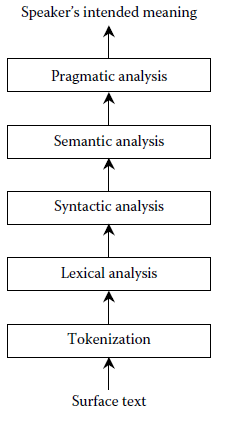
\includegraphics[width=4cm]{pictures/Analyseschritte.png}
\caption{Analyseschritte im klassischen NLP nach \cite[vgl.][4]{DALE}}
\label{fig:STEPS}
\end{wrapfigure}
\par
Den ersten Schritt bildet die \textit{Tokenization}. Zur Vorbereitung des Textes auf die weiteren Analyseschritte werden fundamentale Textbausteine, also Wörtern und Sätzen identifiziert. In segmentierten Sprachen wie dem Englischen, wird das \textit{White-Space-Zeichen} zum separieren der einzelnen Worte genutzt. Komplexe Probleme in diesem Zusammenhang sind beispielsweise die richtige Interpretation der Rolle eines Punktes (Satzende, Abkürzung oder Nummerntrennzeichen), der Umgang mit Mehrwortbenennungen oder die Normalisierung des Textes (Vereinheitlichung von unterschiedlicher Schreibweisen eines Wortes). Hierbei ist die Aussagekraft des Wort- oder Satzkontextes nicht zu unterschätzen. Für die Implementierung der Tokenization existieren zahlreiche regelbasierte Ansätze.
\par
Bei der lexikalische Analyse wird der Text auf Ebene des einzelnen Wortes untersucht. Ein Wort bezeichnet hierbei eine Sammlung von Zeichenfolgen, die zu einem Lemma (Grundform) gehören. Im Rahmen der lexikalischen Analyse wird also eine Zeichenfolge (z.B. singt) in ein Lemma mit morphologischen Zusatzinformationen (z.B. SINGEN, 3. Person Singular Präsens) zugeordnet. Im Vergleich zu anderen Sprachen, in denen durch Flexion zahlreiche komplexe Wortformen entstehen, ist diese Aufgabe im Englischen vergleichsweise einfach. Es stehen außerdem umfangreiche lexikale Ressourcen wie zum Beispiel das \textit{Princeton WordNet} für die lexikalische Analyse zur Verfügung. 
\par
Im Rahmen der syntaktische Analyse wird die grammatische Struktur eines Satzes analysiert. Den einzelnen Satzbausteinen wird ihre Funktion im Satz zugeordnet. Das Ergebnis dieses Zwischenschrittes ist ein Syntaxbaum, in dem sich die Satzstruktur widerspiegelt. Der eingesetzte \textit{Parser} ist im kann bei Mehrdeutigkeit die wahrscheinlichste Interpretation identifizieren.
\par

polysemy!












